\scanpage{125}
% archive sheet number: 124
\[
\begin{aligned}
\sigma_{t_0}:&\quad x\leftrightarrow x',\quad y\leftrightarrow y',\quad z\leftrightarrow z'\\
\sigma_{t\deleted{\unsure{'}}}:&\quad x\leftrightarrow y',\quad y\leftrightarrow z',\quad z\leftrightarrow x'\\
\sigma_{t'}:&\quad x\leftrightarrow z',\quad y\leftrightarrow x',\quad z\leftrightarrow y'
\end{aligned}
\]
\diagram{\resizebox{\linewidth}{!}{\begin{tikzcd}[ampersand replacement=\&,column sep=small,row sep=large]
\sigma_{t_0}\sigma_t: \&x\arrow[r]\&\deleted{\unsure{z}}y\arrow[r]\&\deleted{\unsure{y}}z\arrow[ll,bend right=35]\&x'\arrow[r]\&z'\arrow[r]\&y'\arrow[ll,bend right=35]\&a\arrow[r]\&s\arrow[r]\&s'\arrow[ll,bend right=35]\\
\Vert\&\&\deleted{\unsure{y\longmapsto x}}\\[-1ex]
\sigma_t\sigma_{t'}:\&x\arrow[r]\&y\arrow[r]\&z\arrow[ll,bend right=35]\&x'\arrow[r,no head]\&\unsure{z'}\arrow[r,no head]\&y'\arrow[ll,bend right=35]\&a\arrow[r]\&s\arrow[r]\&s'\arrow[ll,bend right=35]\\
\Vert\\
\sigma_{t'}\sigma_{t_0}:\&\&\&\&\mathrm{id}
\end{tikzcd}}}
\[
\begin{aligned}
&\sigma_{t_0}\sigma_t=\sigma_t\sigma_{t'}=\sigma_{t'}\sigma_{t_0}\deleted{\unsure{=[\sigma_{t_0},\sigma_t]}}=\pi_{a},\quad\pi^3=\mathrm{id}\\
\Downarrow\quad&[\sigma_{t_0},\sigma_t]=[\sigma_t,\sigma_{t'}]=[\sigma_{t'},\sigma_{t_0}]=\pi^2=\pi^{-1})\\
&\sigma_t\sigma_{t_0}=\sigma_{t_0}\sigma_{t'}=\sigma_{t'}\sigma_t=\pi^{-1}\\
\mathrel{\swarrow\!\!\swarrow}\quad&\deleted{\unsure{\sigma_t}}\sigma_{t_0}\sigma_t\sigma_{t'}=\sigma_t\quad\text{etc}
\end{aligned}
\]

$\unsure{\mathfrak S|\mathcal S|\mathcal G}_I$ opère sur $S\unsure{\smallsetminus|-}\underbrace{X}_{\substack{\text{bitriangle}\\\text{plongé}}}$, sans pt fixe (\unsure{orbites}\ \unsure{à} 6 \unsure{élmts}) et \unsure{---} trois orbites, donc trois torseurs sous $\mathfrak S_I$ donc trois ens à trois éléments

\figure{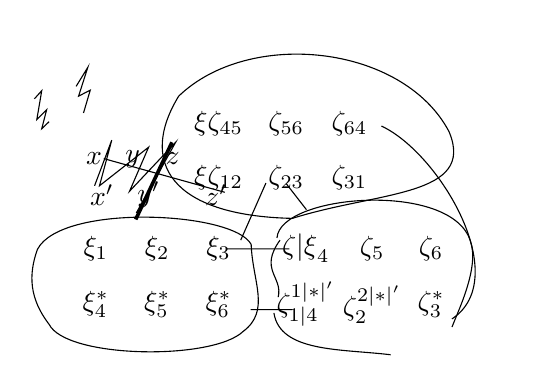
\begin{tikzpicture}[x=.78cm,y=.69cm,every node/.style={inner sep=1pt}]
\draw (2.35,4.45) .. controls (3.5,5.7) and (6.0,5.4) .. (6.75,3.8) .. controls (7.2,2.6) and (5.6,2.7) .. (4.2,2.2) .. controls (2.2,2.25) and (1.7,3.25) .. (2.35,4.45);
\draw (3.95,1.84) .. controls (4.0,2.65) and (6.8,2.9) .. (7.1,1.78) .. controls (7.25,1.3) and (6.9,.5) .. (6.8,.2);
\draw (4.0,1.8) .. controls (3.65,1.25) and (4.05,1.13) .. (3.97,.75);
\draw (3.9,.46) .. controls (4.0,-.27) and (5.0,-.2) .. (5.8,-.31);
\draw (.05,1.63) .. controls (.44,2.48) and (3.25,2.33) .. (3.53,1.72) .. controls (3.55,1.04) and (3.85,.5) .. (3.4,.12) .. controls (2.9,-.42) and (.52,-.38) .. (.24,.25) .. controls (-.08,.72) and (-.1,1.16) .. (.05,1.63);
\foreach \x/\a/\b in {1/1/4,2/2/5,3/3/6}{\node at (\x,1.65){$\xi_{\a}$};\node at (\x,.62){$\xi_{\b}^{*}$};}
\node at (4.42,1.65){$\unsure{\zeta|\xi}_4$};\node at (5.5,1.65){$\zeta_5$};\node at (6.46,1.65){$\zeta_6$};
\node at (4.42,.62){$\zeta_{\unsure{1|4}}^{\unsure{1|*|'}}$};\node at (5.5,.62){$\zeta_2^{\unsure{2|*|'}}$};\node at (6.46,.62){$\zeta_3^{*}$};
\node at (3,3.95){$\deleted{\unsure{\xi}}\zeta_{45}$};\node at (4.1,3.95){$\zeta_{56}$};\node at (5.13,3.95){$\zeta_{64}$};
\node at (3,2.96){$\deleted{\unsure{\xi}}\zeta_{12}$};\node at (4.1,2.96){$\zeta_{23}$};\node at (5.13,2.96){$\zeta_{31}$};
\draw (3.12,1.64)--(4.15,1.64) (3.52,.52)--(4.2,.52) (3.36,1.8)--(3.77,2.85) (4.1,2.84)--(4.43,2.36);
\draw (5.65,3.9) .. controls (6.6,3.4) and (7.8,1.1) .. (6.8,.35);
\node at (.97,3.3){$x$};\node at (1.6,3.28){$\deleted{\unsure{y}}$};\node at (2.25,3.3){$\deleted{\unsure{z}}$};
\node at (1.1,2.63){$x'$};\node at (1.86,2.63){$y'$};\node at (2.96,2.63){$z'$};
\draw (.98,2.8)--(1.26,3.64)--(1.06,2.8)--(1.86,3.51)--(1.55,2.7)--(2.3,3.6)--(1.66,2.3) (1.13,3.3)--(3.1,2.68);
\draw[line width=1.3pt] (1.65,2.18)--(2.24,3.6);
\draw (.0,4.4)--(.12,4.55)--(.04,4.02)--(.2,4.2)--(.12,3.85)--(.24,3.98) (.68,4.63)--(.87,4.98)--(.72,4.45)--(.91,4.56)--(.8,4.14);
\end{tikzpicture}}
\diagram{\begin{tikzcd}[ampersand replacement=\&]
\deleted{X}\arrow[d]\&Z\arrow[d]\&\text{ens à 9 él.}\\
{}\&E\&\text{ens à 3 él.}
\end{tikzcd}}

$I,J$ deux ens à trois él.

$\mathfrak S_I\times\mathfrak S_J$ opère sur ens \deleted{à 18} fini, \inserted{$E$} \deleted{de} façon que $\mathfrak S_I$ et $\mathfrak S_J$ opèrent ss pts fixes, donc \unsure{---} $E=\coprod E_i$, chaque $E_i$ bitorseur sous $\mathfrak S_{\unsure{i|I}}\times\mathfrak S_J$
